\documentclass[aspectratio=169]{beamer}
\usepackage[english]{babel}
\usepackage{booktabs,listings}
\usepackage[T1]{fontenc}
\usepackage[utf8]{inputenc}
\usepackage[style=numeric,backend=bibtex,sorting=none]{biblatex}

\usetheme[slogan=english,mathfont=serif]{NTNU}

\newcommand{\mean}[1]{\left\{\!\!\left\{#1\right\}\!\!\right\}}
\newcommand{\jump}[1]{\left[\!\!\left[ #1 \right]\!\!\right]}
\newcommand{\abs}[1]{\left\lvert #1 \right\rvert}

\addbibresource{bibliography.bib}

\title[Your Short Title]{Cut Finite Element Method for the Cahn-Hilliard Equation}
\subtitle{And why it is quite cool stuff}
\author{Isak Hammer}
\date{\today}

\begin{document}
\maketitle

\section{Introduction}


\begin{frame}{Introducing Myself}
    \begin{columns}
        % Column 1
        \begin{column}{0.5\textwidth}
            \begin{itemize}
                \item Isak Hammer, 27 year old, Lofoten
                \item Graduate student in Industrial Mathematics
                \item Research Focus: Numerical methods for Partial Differential Equations (PDEs).
            \end{itemize}
        \end{column}

        % Column 2
        \begin{column}{0.5\textwidth}
            \begin{figure}
                \centering
                \includegraphics[width=0.7\textwidth]{figures/isak.jpg}
            \end{figure}
        \end{column}
    \end{columns}
\end{frame}

\begin{frame}{Importance and Motivation of the Cahn Hilliard Equation}
    \begin{columns}
        % Column 1
        \begin{column}{0.5\textwidth}
            \begin{itemize}
                \item Thermodynamically modelling of a two-component liquid separation\footnotemark[1].
            \item Modelling of so-called lipid rafts in biological membrane dynamics \footnotemark[2].
            \end{itemize}
        \end{column}
        \begin{column}{0.5\textwidth}
            \begin{itemize}
                \item Droplet dynamics, i.e., coalescence, breakup and movement by coupling with Navier-Stokes \footnotemark[3].
            \end{itemize}
        \end{column}
    \end{columns}
    \footnotetext[1]{\fullcite{cahn1959free}}
    \footnotetext[2]{\fullcite{yushutin2019computational}}
    \footnotetext[3]{\fullcite{zimmermann2019calculation}}
\end{frame}

\begin{frame}
    \begin{block}{The Cahn Hilliard Equation}
        The general Cahn Hilliard Equation  has the form $u( x, t): \Omega \times [0,T] \mapsto [-1,1]   $ s.t.
            \[
            \begin{split}
                 u_t+\Delta\left(\varepsilon \Delta u-\frac{1}{\varepsilon} f(u)\right)&=0 \quad \text{in } \Omega \\
\partial_n u=\partial_n \Delta u& =0 \quad \text{on } \Gamma  \\
 u & =u_0 \quad \text{on } \Omega
            \end{split}
            \]
where $f(s)=F^{\prime}(s)$ and $F(s)=\frac{1}{4}\left(s^2-1\right)^2$ and $\Omega \subset \mathbf{R}^d, d=2,3$, is a bounded domain.
\end{block}

\begin{block}{Challenges}
    \begin{enumerate}
        \item Highly nonlinear and stiff. Often practical applications require $\varepsilon \ll 1$.
        \item 4th order system.
        % \item Conservation of mass and the Neumann conditions conditions.
    \end{enumerate}
\end{block}

\end{frame}

\begin{frame}
    \begin{block}{Why Finite Element Method (FEM)}
        \begin{enumerate}
            \item \textbf{Robust mathematical framework}
            \item \textbf{Can easily handle complex geometries}
            \item \textbf{High flexibility of basis functions}
            \item \textbf{Other: } Supports adaptive refinements, easily adaptable to multi-physics problems ++ .
        \end{enumerate}
    \end{block}
\end{frame}

% \begin{frame}
%     \begin{block}{Strategy to solve the Cahn-Hilliard problem on smooth domains}
%         \begin{enumerate}
%             \item Solve the biharmonic problem $\Delta ^2 u = f$ for polygonal domains.
%             \item Modify the method to handle smooth domains.
%             \item Utilize the time integration to handle non-linearity.
%         \end{enumerate}
%     \end{block}
% \end{frame}

% \begin{frame}
%     \begin{block}{Strategy to solve the Cahn-Hilliard problem on smooth domains}
%         \begin{enumerate}
%             \item First find a suitable method to solve an 4th order PDE for polygonal domains.
%             \item Modify the problem formulation to take account for smooth domains.
%             \item Utilize the time integration to handle nonlinearity.
% \item \textcolor{red}{Make the time-steps small enough or implement adaptivity time schemes.}
%         \end{enumerate}
%     \end{block}
% \end{frame}


% \begin{frame}
% \begin{columns}
% \column{0.55\textwidth}
% \begin{block}{The Biharmonic Problem}
% Let $\Omega \subseteq \mathbb{R} ^d$ be a bounded domain with boundary $\Gamma $ . Let the biharmonic problem have the form s.t. $u:\Omega \mapsto \mathbb{R} $,
% \begin{equation}
% \label{eq:bi_problem}
% \begin{split}
% \Delta^2 u + \alpha u & = f( x) \quad \text{in } \Omega, \\
% \partial_{n} u & = g_{1} \quad \text{on } \Gamma , \\
% \partial_{n} \Delta u & = g_{2} \quad \text{on } \Gamma . \\
% \end{split}
% \end{equation}
% Here is $\Delta ^2 = \Delta \left( \Delta \right) $ the biharmonic operator. The functions $g_{1},g_{2}: \Omega \to \mathbb{R}$ are denoted as boundary conditions.
% \end{block}

% \column{0.45\textwidth}
% \begin{figure}[htpb!]
%     \centering
%     \begin{tikzpicture}
%         % Circle
%         \draw (0.0,0.0) circle (1.5cm);
%         \fill[blue!30] (0.0,0.0) circle (1.5cm);

%         \draw[->, line width=1.0pt] ({1.5*cos(65)}, { 1.5*sin(65) }) -- ({ 2.5*cos(65)  }, { 2.5*sin(65)  }) node[ above left] {$n $};
%         % \draw[->, line width=1.0pt] ({1.5*cos(45)}, { 1.5*sin(45) }) -- ({ 1.5*cos(45) - 1.5*sin(45) }, { 1.5*sin(45) + 1.5*cos(45) }) node[ above right] {$t $};

%         % Labels
%         \node[below right] at (0.5,0.5) {$\Omega$};
%         \node[below right] at (-1.5,-1.2) {$\Gamma$};
%     \end{tikzpicture}
%     \caption{ Illustration of the domain $\Omega $, the boundary $\Gamma $ and the normal vector $n$. }
%     \label{fig:domain_construction}
% \end{figure}
% \end{columns}

% \end{frame}

\begin{frame}
    \frametitle{The Biharmonic Problem (on a polygon)}
    \begin{columns}
        \column{0.55\textwidth}
        \begin{block}{}
            Let $\Omega \approx \Omega_{h} = \mathcal{T}_{h}$ be a bounded \textcolor{red}{polygonal} domain with boundary $\Gamma $ . Let the biharmonic problem have the form s.t. $u:\Omega \mapsto \mathbb{R} $,
            \begin{equation}
                \label{eq:bi_problem}
                \begin{split}
                    \Delta^2 u + \alpha u & = f( x) \quad \text{in } \Omega, \\
                    \partial_{n} u & = 0 \quad \text{on } \Gamma , \\
                    \partial_{n} \Delta u & = 0 \quad \text{on } \Gamma . \\
                \end{split}
            \end{equation}
            Here is $\Delta ^2 = \Delta \left( \Delta \right) $ the biharmonic operator.
        \end{block}

        \column{0.45\textwidth}
        \begin{figure}[htpb!]
            \centering
            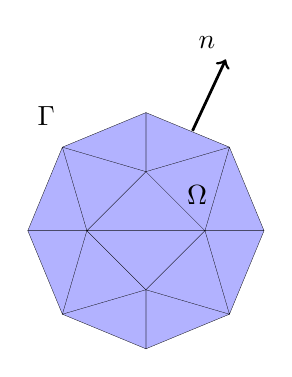
\begin{tikzpicture}
                % FIGURE OF FITTED MESH
                % Boundary points
                \foreach \i in {0, 45, ..., 315} {
                    \coordinate (boundary-\i) at (\i:1.5cm);
                }
                % Interior points
                \coordinate (interior-1) at (0.75, 0);
                \coordinate (interior-2) at (-0.75, 0);
                \coordinate (interior-3) at (0, 0.75);
                \coordinate (interior-4) at (0, -0.75);

                % Create a cycle connecting all the boundary points
                \fill[blue!30] (boundary-0) -- (boundary-45) -- (boundary-90) -- (boundary-135) -- (boundary-180) -- (boundary-225) -- (boundary-270) -- (boundary-315) -- cycle;

                % Labels
                \node[below right] at (0.4,0.7) {$\Omega $};
                \node[below right] at (-1.5,1.7) {$\Gamma $};

                % Triangulation (manually specified)
                \draw[line width=0.1pt] (boundary-0) -- (boundary-45) -- (interior-1) -- cycle;
                \draw[line width=0.1pt] (boundary-45) -- (boundary-90) -- (interior-3) -- cycle;
                \draw[line width=0.1pt] (boundary-90) -- (boundary-135) -- (interior-3) -- cycle;
                \draw[line width=0.1pt] (boundary-135) -- (boundary-180) -- (interior-2) -- cycle;
                \draw[line width=0.1pt] (boundary-180) -- (boundary-225) -- (interior-2) -- cycle;
                \draw[line width=0.1pt] (boundary-225) -- (boundary-270) -- (interior-4) -- cycle;
                \draw[line width=0.1pt] (boundary-270) -- (boundary-315) -- (interior-4) -- cycle;
                \draw[line width=0.1pt] (boundary-315) -- (boundary-0) -- (interior-1) -- cycle;

                % Triangulation between interior points
                \draw[line width=0.1pt] (interior-1) -- (interior-2) -- (interior-3) -- cycle;
                \draw[line width=0.1pt] (interior-1) -- (interior-2) -- (interior-4) -- cycle;

                \draw[->, line width=1.0pt] ({1.4*cos(65)}, { 1.4*sin(65) }) -- ({ 2.4*cos(65)  }, { 2.4*sin(65)  }) node[ above left] {$n $};

            \end{tikzpicture}
            \caption{ Illustration of the mesh $\Omega_{h} $, the boundary $\Gamma $ and the normal vector $n$. }
            \label{fig:domain_construction}
        \end{figure}
    \end{columns}
\end{frame}



\begin{frame}
\frametitle{ $C^0$ Interior Penalty Method (CIP) for the Biharmonic Problem }

\begin{block}{}
The proposed numerical scheme is to find an  $w \in V_{h}$ .t.
\begin{equation*}
\label{eq:CP_A_F}
a_{h}( w, v )   = l_{h}( v) = ( f,v)_{\Omega } , \quad \forall v \in V_{h}  .
\end{equation*}
where
\begin{equation*}
\begin{split}
a_{h} \left( w, v \right)   =&
    \left( \alpha  w, v \right) _{\Omega }   +  \left( \Delta  w, \Delta v \right) _{\Omega } \\
 & +
  \left( \mean{  \Delta  w }, \jump{ \partial _{n }v} \right)_{\mathcal{F}_{h}}  +
 \left( \mean{ \Delta  v }, \jump{ \partial _{n}w }      \right)_{\mathcal{F}_{h}}  + \frac{\gamma }{h}  \left( \jump{ \partial _{n} w}, \jump{ \partial _{n} v   }   \right)_{\mathcal{F}_{h}}
 % l_{h}( v_{h}) & =  \left( f, v \right) _{\Omega }
\end{split}
\end{equation*}

Which is inspired from Brenner2012 \footnotemark[1]
\end{block}

\footnotetext[1]{\fullcite{brenner2012}}

\end{frame}


\begin{frame}
\frametitle{Cut Finite Element Method (CutFEM)}

\begin{block}{Unfitted mesh vs fitted mesh}
    CutFEM is a numerical method for solving partial differential equations (PDEs) using an unfitted mesh.

\begin{figure}
    \centering
    % First TikZ picture
    \begin{minipage}{0.45\textwidth}
        \centering
        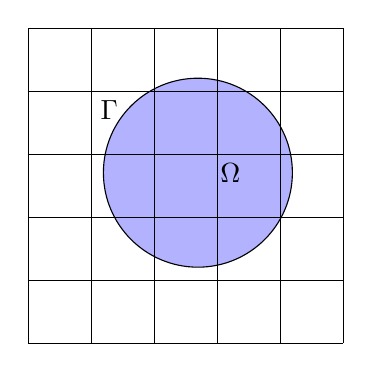
\begin{tikzpicture}[scale=0.80]
            \draw[fill=blue!30] (0.2, 0.2) circle (1.5cm);
            % Background mesh
            \foreach \i in {-2.5, -1.5, ..., 2.5} {
                \draw[line width=0.1pt, shift={(-2.5,\i)}] (0,0) -- (5,0);
                \draw[line width=0.1pt, shift={(\i,-2.5)}] (0,0) -- (0,5);
            }
            % Labels
            \node[below right] at (0.4,0.5) {$\Omega $};
            \node[below right] at (-1.5,1.5) {$\Gamma $};
            % \draw[blue, thick] (-2.5, -2.5) rectangle (2.5, 2.5);
        \end{tikzpicture}
    \end{minipage}
    \hfill
    % Second TikZ picture
    \begin{minipage}{0.45\textwidth}
        \centering
        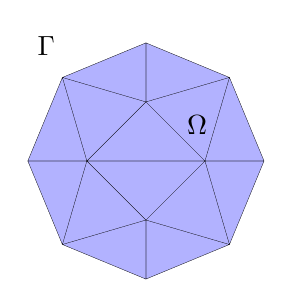
\begin{tikzpicture}[scale=1.0]
            % FIGURE OF UNFITTED MESH
            % Boundary points
            \foreach \i in {0, 45, ..., 315} {
                \coordinate (boundary-\i) at (\i:1.5cm);
            }
            % Interior points
            \coordinate (interior-1) at (0.75, 0);
            \coordinate (interior-2) at (-0.75, 0);
            \coordinate (interior-3) at (0, 0.75);
            \coordinate (interior-4) at (0, -0.75);

            % Create a cycle connecting all the boundary points
            \fill[blue!30] (boundary-0) -- (boundary-45) -- (boundary-90) -- (boundary-135) -- (boundary-180) -- (boundary-225) -- (boundary-270) -- (boundary-315) -- cycle;

            % Labels
            \node[below right] at (0.4,0.7) {$\Omega $};
            \node[below right] at (-1.5,1.7) {$\Gamma $};

            % Triangulation (manually specified)
            \draw[line width=0.1pt] (boundary-0) -- (boundary-45) -- (interior-1) -- cycle;
            \draw[line width=0.1pt] (boundary-45) -- (boundary-90) -- (interior-3) -- cycle;
            \draw[line width=0.1pt] (boundary-90) -- (boundary-135) -- (interior-3) -- cycle;
            \draw[line width=0.1pt] (boundary-135) -- (boundary-180) -- (interior-2) -- cycle;
            \draw[line width=0.1pt] (boundary-180) -- (boundary-225) -- (interior-2) -- cycle;
            \draw[line width=0.1pt] (boundary-225) -- (boundary-270) -- (interior-4) -- cycle;
            \draw[line width=0.1pt] (boundary-270) -- (boundary-315) -- (interior-4) -- cycle;
            \draw[line width=0.1pt] (boundary-315) -- (boundary-0) -- (interior-1) -- cycle;

            % Triangulation between interior points
            \draw[line width=0.1pt] (interior-1) -- (interior-2) -- (interior-3) -- cycle;
            \draw[line width=0.1pt] (interior-1) -- (interior-2) -- (interior-4) -- cycle;

            % \draw[blue, thick] (-2.5, -2.5) rectangle (2.5, 2.5);

        \end{tikzpicture}
    \end{minipage}


    % \caption{Mesh comparison: unfitted mesh (left) adheres to domain and boundary, while fitted mesh (right) employs a triangular mesh for polygonal approximation of the circular domain.}
    \label{fig:domain_mesh}
    \end{figure}
\end{block}

\end{frame}

\begin{frame}
    \frametitle{Cut Finite Element Method}
Background Mesh
    \begin{block}{}
        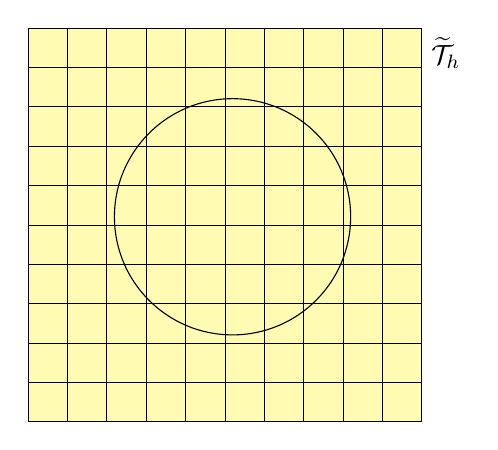
\begin{tikzpicture}[scale=1.0]

            \fill[yellow!30] (-2.5,2.5) -- (2.5,2.5) -- (2.5,-2.5) -- (-2.5,-2.5) -- cycle;

            \draw (0.1, 0.1) circle (1.5cm);
            % Background mesh
            \foreach \i in {-2.5, -2, ..., 2.5} {
                \draw[line width=0.1pt, shift={(-2.5,\i)}] (0,0) -- (5,0);
                \draw[line width=0.1pt, shift={(\i,-2.5)}] (0,0) -- (0,5);
            }


            % Labels
            \node[below right] at (2.5,2.5) {$\widetilde{\mathcal{T}}_{h}$};
        \end{tikzpicture}
    \end{block}
\end{frame}

\begin{frame}
    \frametitle{Cut Finite Element Method}
    Active Mesh
    \begin{block}{}
        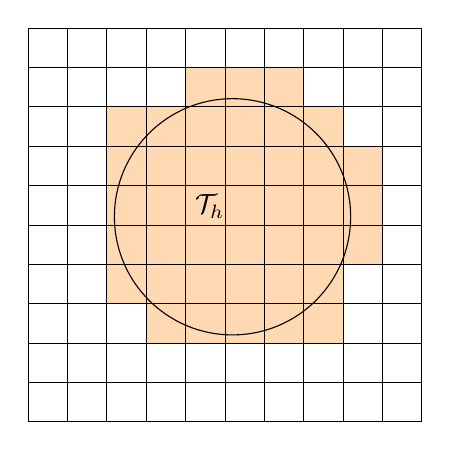
\begin{tikzpicture}[scale=1.0]

            % POTENTIAL ACTIVE MESH
            \fill[orange!30] (2,2) -- (2,-1.5) --(-1.5,-1.5) -- (-1.5,2) -- cycle;

            % ELEMENTS WITH NO INTERSECTION
            % lower left
            \fill[white] (-1.5,-1.5) rectangle (-1.0,-1.0);
            \fill[white] (-1.5,2.0) rectangle (-1.0,1.5);
            \fill[white] (-1.0,2.0) rectangle (-0.5,1.5);
            \fill[white] (2,2) rectangle (1.5,1.5);
            \fill[white] (1.5,2) rectangle (1.0,1.5);
            \fill[white] (2,1.5) rectangle (1.5,1.0);
            \fill[white] (1.5,-1) rectangle (2,-1.5);
            \fill[white] (1.5,-0.5) rectangle (2,-1.0);

            % CUT ELEMENTS
            \fill[orange!30] (-0.5,2.0) rectangle (1.0,1.5);
            \fill[orange!30] (-1.5,1.5) rectangle (0.0,1.0);
            \fill[orange!30] (0.5,1.5) rectangle (1.5,1.0);
            \fill[orange!30] (-1.5,1.0) rectangle (-1.0,-1.0);
            \fill[orange!30] (-1.0,-0.5) rectangle (-0.5,-1.5);
            \fill[orange!30] (-0.5,-1.5) rectangle (1.5,-1.0);
            \fill[orange!30] (1.5,-1) rectangle (1.0,-0.0);
            \fill[orange!30] (1.5,-0.5) rectangle (2.0,1.0);
            \fill[orange!30] (1.0,0.5) rectangle (1.5,1.0);

            \draw (0.1, 0.1) circle (1.5cm);
            % Background mesh
            \foreach \i in {-2.5, -2, ..., 2.5} {
                \draw[line width=0.1pt, shift={(-2.5,\i)}] (0,0) -- (5,0);
                \draw[line width=0.1pt, shift={(\i,-2.5)}] (0,0) -- (0,5);
            }


            % Labels
            % \node[below right] at (2.5,2.5) {$\widetilde{\mathcal{T}}_{h}$};
            % \node[below right] at (0.4,0.5) {$\mathcal{T}_{int}$};
            \node[below right] at (-0.5,0.5) {$\mathcal{T}_{h }$};
        \end{tikzpicture}
    \end{block}
\end{frame}

\begin{frame}
    \frametitle{Cut Finite Element Method}
    Interior Mesh and Cut Cells
    \begin{block}{}
        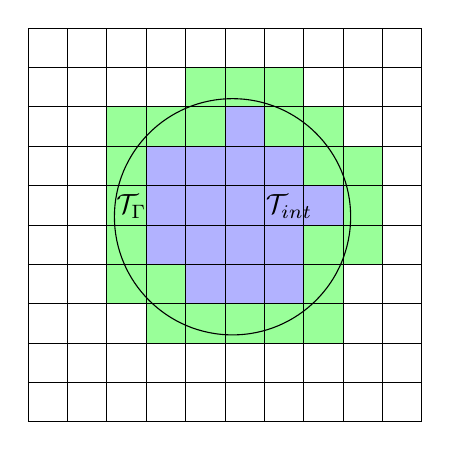
\begin{tikzpicture}[scale=1]

            % POTENTIAL ACTIVE MESH
            \fill[blue!30] (2,2) -- (2,-1.5) --(-1.5,-1.5) -- (-1.5,2) -- cycle;

            % ELEMENTS WITH NO INTERSECTION
            % lower left
            \fill[white] (-1.5,-1.5) rectangle (-1.0,-1.0);
            \fill[white] (-1.5,2.0) rectangle (-1.0,1.5);
            \fill[white] (-1.0,2.0) rectangle (-0.5,1.5);
            \fill[white] (2,2) rectangle (1.5,1.5);
            \fill[white] (1.5,2) rectangle (1.0,1.5);
            \fill[white] (2,1.5) rectangle (1.5,1.0);
            \fill[white] (1.5,-1) rectangle (2,-1.5);
            \fill[white] (1.5,-0.5) rectangle (2,-1.0);

            % CUT ELEMENTS
            \fill[green!40] (-0.5,2.0) rectangle (1.0,1.5);
            \fill[green!40] (-1.5,1.5) rectangle (0.0,1.0);
            \fill[green!40] (0.5,1.5) rectangle (1.5,1.0);
            \fill[green!40] (-1.5,1.0) rectangle (-1.0,-1.0);
            \fill[green!40] (-1.0,-0.5) rectangle (-0.5,-1.5);
            \fill[green!40] (-0.5,-1.5) rectangle (1.5,-1.0);
            \fill[green!40] (1.5,-1) rectangle (1.0,-0.0);
            \fill[green!40] (1.5,-0.5) rectangle (2.0,1.0);
            \fill[green!40] (1.0,0.5) rectangle (1.5,1.0);

            \draw (0.1, 0.1) circle (1.5cm);
            % Background mesh
            \foreach \i in {-2.5, -2, ..., 2.5} {
                \draw[line width=0.1pt, shift={(-2.5,\i)}] (0,0) -- (5,0);
                \draw[line width=0.1pt, shift={(\i,-2.5)}] (0,0) -- (0,5);
            }


            % Labels
            \node[below right] at (0.4,0.5) {$\mathcal{T}_{int}$};
            \node[below right] at (-1.5,0.5) {$\mathcal{T}_{\Gamma }$};
        \end{tikzpicture}
    \end{block}
\end{frame}

\begin{frame}
\frametitle{Cut Finite Element Method (CutFEM)}

A recent and promising numerical technique for PDEs, has gained significant momentum in the past decade \footnotemark[1]\footnotemark[2].

\begin{block}{}
    \begin{itemize}
        \item  Complex domains and moving domains efficiently.
        \item Utilizing so-called ghost penalties to ensure well-posedness.
        % \item Dividing the computational domains into \textbf{background} , \textbf{active}, \textbf{cut}  and \textbf{interior} mesh.
    \end{itemize}
\end{block}
\footnotetext[1]{\fullcite{burman2015cutfem}}
\footnotetext[2]{\fullcite{gurkan2019stabilized}}

\end{frame}




% \begin{frame}
% \frametitle{ Cut $C^0$ Interior penalty method (CutCIP) }

% \begin{block}{}
% The discretized numerical problem is to solve $w \in V_{h}$ such that
% \begin{equation*}
% \label{eq:CP_A_F}
% A( w, v )  = a_{h}( w,v) + \textcolor{red}{g_{h}( w,v)}  = l_{h}( v), \quad \forall v \in V_{h}  .
% \end{equation*}

% Where the additional bilinear term $g_{h}( w,v) : V_{h} \times V_{h} \to  \mathbb{R} $ is the so-called \textbf{ghost penalty}, which does the numerical regularization to ensure stability on cut cells.

% \end{block}

% \end{frame}

\begin{frame}
\frametitle{ CutCIP Method}

My master's thesis is dedicated to demonstrating that the relevant properties remain valid for CutCIP formulation still holds.

    \begin{block}{Well-posedness }
         The discrete bilinear form $a_{h}$ is wellposed on $V_{h}$ if this holds; \[
             \begin{split}
                 (Coercivity) \quad  A( v,v) &  \gtrsim  \| v \|_{A }^{ 2 } \quad  \forall v \in  V_{h} \\
            (Boundedness) \quad A( v,w) & \lesssim  \| v \|_{A }^{  }\| w \|_{a_{h} }^{  } \quad  \forall v,w \in  V_{h}
             \end{split}
        \]
    \end{block}

    \begin{block}{Apriori Estimates }

         Let $u$ be the solution to the strong problem with the corresponding discrete solution $u_{h}$ with polynomical order $k\ge 2$ .
        Then does it exist  $l = \min_{} ( 2, k)  $ s.t.
\[
        \| u - u_{h} \|_{a_{h}  }^{  } \lesssim  h^{l-1} \| u \|_{ H^{l} ( \Omega ) }^{  }
\]
    \end{block}
    % \footnotetext[1]{\fullcite{Gu2012}}
\end{frame}



\begin{frame}
\frametitle{ Cut $C^0$ Interior Penalty Method (CutCIP) Results }
% \frametitle{Manufactured Solution}


\begin{block}{Manufactured solution}
    In the experiments will we only consider polynomial order $k=2$.
We consider the manufactured solution:
$$
u_{ex}(\mathbf{x}) = \left(x_1^2 + x_2^2 - 1\right)^2 \cos(2\pi x_1) \cos(2\pi x_2)
$$
where $\mathbf{x}=(x_1,x_2)$ and $\Omega=\{(x_1,x_2): x_1^2 + x_2^2 \le  1\}$.
This manufactured solution can be used to test the accuracy of numerical methods for solving the above differential equation.
\end{block}
\end{frame}


\begin{frame}
\frametitle{ Cut $C^0$ Interior penalty method (CutCIP) Results }
\resizebox{\textwidth}{!}{
\begin{tabular}{rrrrrrrrr}
    \hline\hline
    \textbf{$n$} & \textbf{$\Vert e \Vert_{L^2}$} & \textbf{EOC} & \textbf{$ \Vert e \Vert_{H^1}$} & \textbf{EOC} & \textbf{$\Vert e \Vert_{ a_h,* }$} & \textbf{EOC} & \textbf{Cond number} & \textbf{ndofs} \\\hline
    4 & 2.4E+00 &  & 3.3E+00 &  & 6.2E+01 &  & 8.7E+04 & 8.1E+01 \\
    8 & 3.6E-01 & 2.72 & 1.1E+00 & 1.60 & 3.9E+01 & 0.68 & 5.1E+05 & 2.4E+02 \\
    16 & 2.2E-02 & 4.06 & 2.5E-01 & 2.12 & 1.4E+01 & 1.51 & 3.7E+06 & 8.3E+02 \\
    32 & 5.6E-03 & 1.97 & 6.0E-02 & 2.04 & 3.6E+00 & 1.93 & 2.8E+07 & 3.0E+03 \\
    64 & 1.4E-03 & 2.00 & 1.5E-02 & 2.02 & 9.2E-01 & 1.96 & 2.1E+08 & 1.1E+04 \\
    128 & 3.5E-04 & 2.00 & 3.7E-03 & 2.01 & 2.4E-01 & 1.94 & 1.7E+09 & 4.3E+04 \\\hline\hline
  \end{tabular}
}
\end{frame}






\begin{frame}
\frametitle{ Cut $C^0$ Interior penalty method (CutCIP) Results }

\begin{figure}[h!]
    \centering
    \resizebox{0.6\textwidth}{!}{% Recommended preamble:
% \usetikzlibrary{arrows.meta}
% \usetikzlibrary{backgrounds}
% \usepgfplotslibrary{patchplots}
% \usepgfplotslibrary{fillbetween}
% \pgfplotsset{%
%     layers/standard/.define layer set={%
%         background,axis background,axis grid,axis ticks,axis lines,axis tick labels,pre main,main,axis descriptions,axis foreground%
%     }{
%         grid style={/pgfplots/on layer=axis grid},%
%         tick style={/pgfplots/on layer=axis ticks},%
%         axis line style={/pgfplots/on layer=axis lines},%
%         label style={/pgfplots/on layer=axis descriptions},%
%         legend style={/pgfplots/on layer=axis descriptions},%
%         title style={/pgfplots/on layer=axis descriptions},%
%         colorbar style={/pgfplots/on layer=axis descriptions},%
%         ticklabel style={/pgfplots/on layer=axis tick labels},%
%         axis background@ style={/pgfplots/on layer=axis background},%
%         3d box foreground style={/pgfplots/on layer=axis foreground},%
%     },
% }

\begin{tikzpicture}[/tikz/background rectangle/.style={fill={rgb,1:red,1.0;green,1.0;blue,1.0}, fill opacity={1.0}, draw opacity={1.0}}, show background rectangle]
\begin{axis}[point meta max={nan}, point meta min={nan}, legend cell align={left}, legend columns={1}, title={}, title style={at={{(0.5,1)}}, anchor={south}, font={{\fontsize{14 pt}{18.2 pt}\selectfont}}, color={rgb,1:red,0.0;green,0.0;blue,0.0}, draw opacity={1.0}, rotate={0.0}, align={center}}, legend style={color={rgb,1:red,0.0;green,0.0;blue,0.0}, draw opacity={1.0}, line width={1}, solid, fill={rgb,1:red,1.0;green,1.0;blue,1.0}, fill opacity={1.0}, text opacity={1.0}, font={{\fontsize{8 pt}{10.4 pt}\selectfont}}, text={rgb,1:red,0.0;green,0.0;blue,0.0}, cells={anchor={center}}, at={(1.02, 1)}, anchor={north west}}, axis background/.style={fill={rgb,1:red,1.0;green,1.0;blue,1.0}, opacity={1.0}}, anchor={north west}, xshift={1.0mm}, yshift={-1.0mm}, width={94.6mm}, height={74.2mm}, scaled x ticks={false}, xlabel={$\delta$}, x tick style={color={rgb,1:red,0.0;green,0.0;blue,0.0}, opacity={1.0}}, x tick label style={color={rgb,1:red,0.0;green,0.0;blue,0.0}, opacity={1.0}, rotate={0}}, xlabel style={at={(ticklabel cs:0.5)}, anchor=near ticklabel, at={{(ticklabel cs:0.5)}}, anchor={near ticklabel}, font={{\fontsize{11 pt}{14.3 pt}\selectfont}}, color={rgb,1:red,0.0;green,0.0;blue,0.0}, draw opacity={1.0}, rotate={0.0}}, xmajorgrids={true}, xmin={-0.001471665988344504}, xmax={0.05052719893316125}, xticklabels={{$0.00$,$0.01$,$0.02$,$0.03$,$0.04$,$0.05$}}, xtick={{0.0,0.010000000000000002,0.020000000000000004,0.030000000000000006,0.04000000000000001,0.05000000000000001}}, xtick align={inside}, xticklabel style={font={{\fontsize{8 pt}{10.4 pt}\selectfont}}, color={rgb,1:red,0.0;green,0.0;blue,0.0}, draw opacity={1.0}, rotate={0.0}}, x grid style={color={rgb,1:red,0.0;green,0.0;blue,0.0}, draw opacity={0.1}, line width={0.5}, solid}, axis x line*={left}, x axis line style={color={rgb,1:red,0.0;green,0.0;blue,0.0}, draw opacity={1.0}, line width={1}, solid}, scaled y ticks={false}, ylabel={$\kappa(A)$}, y tick style={color={rgb,1:red,0.0;green,0.0;blue,0.0}, opacity={1.0}}, y tick label style={color={rgb,1:red,0.0;green,0.0;blue,0.0}, opacity={1.0}, rotate={0}}, ylabel style={at={(ticklabel cs:0.5)}, anchor=near ticklabel, at={{(ticklabel cs:0.5)}}, anchor={near ticklabel}, font={{\fontsize{11 pt}{14.3 pt}\selectfont}}, color={rgb,1:red,0.0;green,0.0;blue,0.0}, draw opacity={1.0}, rotate={0.0}}, ymode={log}, log basis y={10}, ymajorgrids={true}, ymin={100000.0}, ymax={1.0e25}, yticklabels={{$10^{5}$,$10^{10}$,$10^{15}$,$10^{20}$,$10^{25}$}}, ytick={{100000.0,1.0e10,1.0e15,1.0e20,1.0e25}}, ytick align={inside}, yticklabel style={font={{\fontsize{8 pt}{10.4 pt}\selectfont}}, color={rgb,1:red,0.0;green,0.0;blue,0.0}, draw opacity={1.0}, rotate={0.0}}, y grid style={color={rgb,1:red,0.0;green,0.0;blue,0.0}, draw opacity={0.1}, line width={0.5}, solid}, axis y line*={left}, y axis line style={color={rgb,1:red,0.0;green,0.0;blue,0.0}, draw opacity={1.0}, line width={1}, solid}, colorbar={false}]
    [\addlegendimage{empty legend}] \addlegendentry[font={{\fontsize{11 pt}{14.3 pt}\selectfont}}, text={rgb,1:red,0.0;green,0.0;blue,0.0}] {\hspace{-.6cm}{\textbf{$(\gamma, \gamma_1, \gamma_2)$}}}
    \addplot[color={rgb,1:red,0.0;green,0.0;blue,1.0}, name path={e73f70a5-bbbd-4a24-8407-eef9d08bc09d}, draw opacity={1.0}, line width={1}, solid]
        table[row sep={\\}]
        {
            \\
            0.0  1.2679164207221107e8  \\
            0.012263883236204186  1.2718633484176141e8  \\
            0.024527766472408372  1.2693944128424127e8  \\
            0.03679164970861256  1.2718633338545807e8  \\
            0.049055532944816745  1.2679164340263365e8  \\
        }
        ;
    \addlegendentry { $1.0 \cdot 10^{1}$, $0.5 \cdot 10^{1}$, $1.0 \cdot 10^{-1}$ }
    \addplot[color={rgb,1:red,1.0;green,0.0;blue,0.0}, name path={8dbacc37-3690-4b1f-9d5d-1b6f1fc900ac}, draw opacity={1.0}, line width={1}, solid]
        table[row sep={\\}]
        {
            \\
            0.0  4.639960110962716e10  \\
            0.012263883236204186  4.932252358128007e12  \\
            0.024527766472408372  4.0959531093983247e12  \\
            0.03679164970861256  4.932252223523245e12  \\
            0.049055532944816745  4.639960117645048e10  \\
        }
        ;
    \addlegendentry { $1.0 \cdot 10^{1}$, $ 0.0 \cdot 10^{0} $, $ 0.0 \cdot 10^{0} $ }
\end{axis}
\end{tikzpicture}
}
    \caption{The plot presents the $L^2$ and $H^1$ error norms and the error in the energy norm ($\Vert e \Vert_{a_h,*}$).}
    \label{fig:CutFEM_error1}
\end{figure}

\end{frame}

\begin{frame}
\frametitle{The Cahn Hilliard Equation}
    \begin{columns}
        % Left column
        \begin{column}{0.5\textwidth}
            \begin{block}{Recall}
                The problem has the form $u( x, t): \Omega \times [0,T] \mapsto [-1,1]$ s.t.
                \[
                \begin{split}
                    u_t+\Delta\left(\varepsilon \Delta u-\frac{1}{\varepsilon} f(u)\right)&=0 \quad \text{in } \Omega \\
                    \partial_n u=\partial_n \Delta u& =0 \quad \text{on } \Gamma  \\
                    u & =u_0 \quad \text{on } \Omega
                \end{split}
                \]
                where $f(u)$ is a nonlinear function.
            \end{block}
        \end{column}
        % Right column
        \begin{column}{0.5\textwidth}
            \begin{block}{Plan forward}
                \begin{enumerate}
                    \item We have now a tool to solve the $\Delta ( \Delta u) $ operator
                    \item Will utilize the time-iteration scheme to solve non-linearity
                \end{enumerate}
            \end{block}
        \end{column}
    \end{columns}
\end{frame}


\begin{frame}
\frametitle{The CutCIP Cahn-Hilliard Formulation}


Drawing upon the concepts delineated in Feng\footnotemark[1], the most efficient approach to address the nonlinear term is by employing an implicit-explicit (IMEX) scheme.

\begin{block}{IMEX method on the CutCIP formulation}
    Let $u^{m}_{h} \in V_{h}$ for the timesteps $m=0,1,\ldots,M$. Let $u_{h}^{0} = u_{0}$ be the initial timestep, then is.
\[
(\overline{\partial}  _{t} u_{h}^m, v_h ) + \varepsilon A (u_{h}^{m}, v_h )+\frac{1}{\varepsilon} c_h ( u_{h}^{m-1}, v_h)=0 \quad \forall v_h \in V_h^m .
\]
Here is $c_{h}( . , .) $ an the nonlinear terms handled in a implicit fashion. The $ \overline{\partial}  _{t}$ operator is simply a finite difference scheme in time-dimension.

\end{block}

\footnotetext[1]{\fullcite{feng2007fully}}
\end{frame}

\begin{frame}
\frametitle{The CutCIP Cahn-Hilliard Experiments}
Implemented using the Gridap FEM framework written in Julia \footnotemark[1].


\begin{block}{Simulation parameters}
    \begin{itemize}
        \item Physical domain $\Omega$  is a 4 discs of radius $R=1$ with distance $d=0.999$, i.e. they are touching!
        \item Inital data is $u_0 = random(-1,1)$ in physical domain $\Omega $.
        % \item Backgroundmesh with size ($L\times L$ ) for $L=2$ and $n=128$.
        % \item Polynomial order $k=2$ .
        % \item Physical parameter $\varepsilon  = \frac{1}{30}$.
        % \item Time-step $\tau = \varepsilon ^{2} \frac{1}{10} $ for the interval $ 0\le t \le 10^3 \tau $.
    \end{itemize}
\end{block}

\footnotetext[1]{\fullcite{badia2020gridap}}


\end{frame}

\begin{frame}
\frametitle{The CutCIP Cahn-Hilliard Experiments}

\begin{figure}[h]
    \centering
    \includegraphics[width=0.5\textwidth]{CH-example/0.png}
    \caption{Iteration 0}
    \label{fig:your_image_label}
\end{figure}
\end{frame}

\begin{frame}
\frametitle{The CutCIP Cahn-Hilliard Experiments}

\begin{figure}[h]
    \centering
    \includegraphics[width=0.5\textwidth]{CH-example/1.png}
    \caption{Iteration 1}
\end{figure}
\end{frame}

\begin{frame}
\frametitle{The CutCIP Cahn-Hilliard Experiments}
\begin{figure}[h]
    \centering
    \includegraphics[width=0.5\textwidth]{CH-example/10.png}
    \caption{Iteration 10}
\end{figure}
\end{frame}

\begin{frame}
\frametitle{The CutCIP Cahn-Hilliard Experiments}
\begin{figure}[h]
    \centering
    \includegraphics[width=0.5\textwidth]{CH-example/50.png}
    \caption{Iteration 50}
\end{figure}
\end{frame}

\begin{frame}
\frametitle{The CutCIP Cahn-Hilliard Experiments}
\begin{figure}[h]
    \centering
    \includegraphics[width=0.5\textwidth]{CH-example/200.png}
    \caption{Iteration 200}
\end{figure}
\end{frame}

\begin{frame}
\frametitle{The CutCIP Cahn-Hilliard Experiments}
\begin{figure}[h]
    \centering
    \includegraphics[width=0.5\textwidth]{CH-example/1000.png}
    \caption{Iteration 1000}
\end{figure}
\end{frame}


\begin{frame}
\frametitle{Further work}
\begin{enumerate}
    \item Adaptive time steps.
    \item Further numerical validation.
    \item Extend the method to handle moving domains.

\end{enumerate}
\end{frame}


\begin{frame}
\frametitle{Questions?}
\end{frame}



% % intro


\newpage
\section{Finite Element Method}%
\label{sec:finite_element_method}


\begin{frame}{}
        \begin{block}{Finite Element Methods!}
            \begin{itemize}
                \item To simplify will I only consider Poisson equation $ \Delta u =f $
                    \begin{itemize}
                        \item However, same ideas applies to Navier-Stokes and Cahn-Hilliard
                    \end{itemize}
                \item But to tell the story we need to do math
                    \begin{itemize}
                        \item Notation, inverse inequalities, variational forms, domains etc
                        \item \textbf{I will skip a lot of details,} but still promote the main ideas.
                    \end{itemize}
            \end{itemize}
        \end{block}
\end{frame}

\begin{frame}{}
        \begin{block}{We start with finite difference}
            \begin{itemize}
                \item Then we gradually introduce flaws and problems!
            \end{itemize}
        \end{block}
\end{frame}

\begin{frame}{Poisson Problem}
    Let us define the physical domain $\Omega  \subset \mathbb{R} ^{2}$ and the scalar functions $f: \Omega  \to \mathbb{R}$ and $g: \Omega  \to \mathbb{R} $.
        \begin{block}{Poisson Problem}
  We define the strong formulation of the Possion problem to find a scalar solution
 $u:\Omega  \to \mathbb{R} $ s.t. \[
\begin{split}
    -\Delta u &= f \quad  \text{in }\Omega  \\
     u &= g  \quad \text{on } \Gamma      \\
\end{split} .
\]
        \end{block}
\end{frame}

\begin{frame}{}
        \begin{block}{Finite difference approach}
            \begin{itemize}
                \item Taylor expansion in $y$ and $x$ direction. \[
                        \begin{split}
                \Delta u & = u_{xx} + u_{yy} \\
                & \approx  \frac{u( x-h, y) - 2u( x,y) + u( x +h,y)   }{h^2} + \frac{u( x, y-h) - 2u( x,y) + u( x,y +h)   }{h^2}
                        \end{split}
                \]
            \item Works very well for perfectly square domains
                \begin{figure}
                    \centering
                    \includegraphics[width=0.35 \textwidth]{figures/fdm.png}
                \end{figure}
            \end{itemize}
        \end{block}
\end{frame}

\begin{frame}{}
        \begin{block}{Finite difference approach}
            \begin{itemize}
            \item Can be very messy for unstructured mesh!
                \begin{figure}
                    \centering
                    \includegraphics[width=0.35 \textwidth]{figures/triangulation.png}
                \end{figure}
            \item It does exists methods for handling nodes on these domains.
                \begin{itemize}
                    \item The implementation can be very messy
                    \item Does not scale that well as far as I know.
                \end{itemize}
            \end{itemize}
        \end{block}
\end{frame}


\begin{frame}{Finite element method}
        \begin{block}{Finite element approach for triangulations}
            \begin{enumerate}
                \item We want to write the problem on a equivalent integral form.
                \item Introduce so-called test functions space
                \item Introduce a discrete polynomial space as an approximation space.
            \end{enumerate}
        \end{block}
\end{frame}

\begin{frame}{Finite element method}

        \begin{block}{Let us introduce some notation}
            \begin{itemize}
                \item
                 Function spaces
                    \begin{equation*}
                        \begin{split}
                        L^{2}( \Omega  ) & = \left\{ f: \Omega \mapsto \mathbb{R}  \mid \int_{\Omega }^{} \left\lvert f \right\rvert ^{2} d \Omega  < \infty  \right\} \\
                        H^{1}( \Omega  ) & = \left\{ u \in L^{2}\left( \Omega  \right)  \text{ and }  \nabla  u \in L^{2}\left( \Omega  \right)   \right\}.
                        \end{split}
                    .\end{equation*}

                \item Essentially is $L^2( \Omega ) $ the space of all integrable functions.
                    \begin{itemize}
                        \item \textbf{Example:} $ \int_{-1}^{1} (\frac{1}{x}) dx  $ is not $L^2(\left[ -1,1 \right] )$  integrable. \\
                        \item \textbf{Example:} $ \int_{2}^{3} (\frac{1}{x}) dx  $ is $L^2(\left[ 2,3 \right] )$  integrable. \\
                    \end{itemize}


                \item $H^{1}( \Omega )$ is the space off all functions where both the function and its first derivative is integrable.
            \end{itemize}

        \end{block}
\end{frame}


\begin{frame}{Finite element method}

        \begin{block}{Norms and inner products}
            \begin{itemize}
                \item For $u ,v \in L^2( \Omega )  $ we define  \[
                        \begin{split}
\| u \|_{  \Omega   }^{  } & = \| u \|_{ L^{2}\left( \Omega  \right)  }^{  }   = \left( \int_{\Omega }^{} \left\lvert u \right\rvert ^{2} dx  \right) ^{\frac{1}{2}} \\
\left( u,v \right) _{\Omega } & = \left( u,v \right) _{L^2\left( \Omega  \right) } = \int_{\Omega }^{} u  v dx. \\
                        \end{split}
                    \]
                \item  For $u,v \in H^1( \Omega ) $ we define \[
                    \begin{split}
\| u \|_{ H^{1}\left( \Omega  \right)  }^{  }  & =  \| u \|_{ \Omega } +\| \nabla u \|_{ \Omega }    , \\
\left( u,v \right) _{H^{1}( \Omega )  } & = \left( u,v \right) _{\Omega  } + \left( \nabla u, \nabla v \right) _{\Omega  }
                    \end{split} .
                    \]
            \end{itemize}

        \end{block}

\end{frame}


\begin{frame}{Finite element method}
        \begin{block}{Writing the Poission problem on an integral form   }
            \begin{enumerate}
                \item We extent the definitions for the boundary conditions s.t.
                    \begin{itemize}
                        \item $H^{1}_{0} = \left\{ v \in H^{1 }( \Omega )   \mid  v = 0 \text{ on } \Gamma   \right\} $
                        \item  $V_{g} = \left\{ v \in H^{1 }( \Omega )   \mid  u = g \text{ on }  \Gamma   \right\} $
                    \end{itemize}
                    Notice that the boundary conditions is built in to the space!
                \item Let $u \in V_{g}$. If we multiply with a so-called test function $v \in H^{1}_{0}( \Omega ) $ and apply Greens theorem we get
                    \[
                - \int_\Omega  \Delta u v dx  = \int_\Omega  \nabla u \nabla v dx - \int_\Gamma \partial _{n} u v dx  =  \int_\Omega  \nabla u \nabla v dx
                    \]

                    We will use the following compact notation:
                    \[
                -( \Delta u, v) _{\Omega } = ( \nabla u, \nabla v)_{\Omega} - (\partial _{n} u, v )_{\Gamma }  =  ( \nabla u, \nabla v)_{\Omega}
                \]

            \end{enumerate}
        \end{block}
\end{frame}

\begin{frame}{Finite element method}
        \begin{block}{Writing the Poission problem on an integral form  }
             Let us denote a bilinear form and a linear form \[
            a( u,v)  := ( \nabla u,\nabla v)_{\Omega } \text{ and }  \quad l ( v) := ( f,v) _{\Omega  }
            \]
            The weak formulation of the Poisson problem is to find a $u \in V_{g}$ s.t. \[
            a( u,v) = l ( v) \quad  \forall v  \in  H^{1}_{0}( \Omega  )
            \]

        \end{block}

        How can we discretize the following function spaces?
\end{frame}

\begin{frame}{Abstract definition of a finite element}
    \begin{block}{}
    We define a element as the triple $(T, \mathcal{P}, \Sigma )$ where,
    \begin{itemize}
        \item $T$ is an triangle
        \item $\mathcal{P}^{k}( T)   $ is a finite polynomial basis $\left\{ \phi  \right\}_{i}^{n} $  of dimension $k$, also known as shape functions.
        \item $\Sigma $ is the dual of $\mathcal{P}^{k}( T)  $, that is, the set of linear forms $\left\{ \sigma _{i} \right\}_{i}^{n} $ with the mapping,
            \[
            \sigma _{i}:  \mathcal{P}^{k}( T) \to \mathbb{R} \quad  \text{ such that  } \quad   \sigma _{i}( \phi _{j})  = \delta _{ij}
            \]
            Also contains the DOFs or the coefficients in the polynom!
    \end{itemize}
    \end{block}

    \textbf{Example:} For $k=1$ the DOF in a triangle is one coefficient per mesh node, i.e., number of DOFs is $n = 3$.


\end{frame}

\begin{frame}{Finite element method}
    The absolute key idea of the finite element methods is the following; \\
    \begin{itemize}
        \item \textbf{ The goal is to approximate the (infinite dimensial) function space $H^{1}( \Omega ) $ with a finite dimensional polynomial space $\mathcal{P}^{k}( \Omega ) = span  \left\{ \phi_{1}, \ldots, \phi _{N}  \right\} $ of order $k$  }
    \end{itemize}

\end{frame}

\begin{frame}{Finite element method}
    To solve the Poisson problem using FEM we have the following discrete problem;

    \begin{block}{ Discrete Poisson problem }
    We want to find an $u_{h} \in V_{h} := \mathcal{P}^{k}( \Omega )  $ s.t. \[
    a( u_{h}, v_{h}) = l ( v_{h}) \quad  \forall v_{h} \in V_{h}
    \]
    \end{block}

\end{frame}

\begin{frame}{Finite element method}

    \begin{block}{ Constructing the linear system  }
        \begin{itemize}
            \item Since $v_{h}, u_{h} \in V_{h} := \mathcal{P}^{k}( \Omega )  $ can we write $u_{h} = \sum_{i=0}^{N} U_{i} \phi _{i} $ and $v_{h} = \sum_{i=0}^{N} U_{i} \phi _{i} $ with coefficients $\left\{ U_{i} \right\}_{i=0} ^{N} $ and $\left\{ V_{i} \right\}_{i=0} ^{N} $.
        \item Let us define a matrix $\left[ \mathcal{A}  \right] _{ji} = a( \phi_{i}, \phi _{j} ) $ and $\left[ F \right] _{j} = l( \phi _{j})   $.
        \end{itemize}
    \end{block}
    Thus, we have \[
    \sum_{i,j}^{N} V_{j} U_{i}\ a( \phi_{j}, \phi _{i} ) =  \sum_{j}^{N} V_{j}\ l(\phi _{j})     .
    \]
    Hence, we have the following equivalent linear system, that is \[
    \mathcal{A} U = F.
    \]
\end{frame}

\begin{frame}{Energy norm}

   We will now show requirements for uniqueness of numerical solution, but we need the so-called energy norm.

   \begin{block}{  }
    The energy norm  is denoted by  \[
    \| v \|_{a  }^{ 2 } = a( v,v)
    \]
    \end{block}



\end{frame}

\begin{frame}{Requirements for a well-posed problem}
    \begin{theorem}[ The (discrete) Lax-Milgram Theorem]
        Assume we have a general the bilinear form  $a_{h}: V_{h} \times V_{h} \to \mathbb{R}  $ and a bounded linear form $l_{h}: V_{h} \to \mathbb{R} $. If there exists some constants $C_{1} >0$ and $C_{2} >0$  such that;
        \begin{enumerate}
            \item The bilinear form is bounded,
                \[
                      \abs{a_{h}( v,w)  }    \le C_{1} \| v \|_{a_{h}  }^{  }  \| w \|_{a_{h}  }^{  } \quad \forall v,w  \in V_{h}.
                \]
            \item The bilinear form is coercive (one-to-one), \[
           a_{h}( v,v) \ge  C_{2} \| v \|_{ a_{h} }^{  2} \quad \forall v \in V_{h}.
            \]
        \end{enumerate}
        then it exists a unique discrete solution $u \in V_{h}$ s.t. \[
        a_{h}( u,v)  = l_{h}( v) \quad  \forall v \in V_{h}
        \]
    \end{theorem}


\end{frame}

\begin{frame}{Why is a well-posed problem so interesting?}
    \begin{block}{ Consequences of Lax Milgram }
    \begin{enumerate}
        \item The solution is accurate and reliable.
        \item The discrete problem converges when $h\to 0$
        \item Does not exists infinite solutions
        \item The problem is stable respect to small perturbation.
    \end{enumerate}

    \end{block}
    \begin{block}{Conclusion}
        \begin{itemize}
            \item Lax-Milgram very useful and rigour tool when developing new FEM schemes.
            \item Still hard to apply directly nonlinear problems, but we use it as a basis on simplified problems before we introduce nonlinear terms.
                \begin{enumerate}
                    \item Stokes equation vs Navier Stokes equation
                    \item Biharmonic equation vs Chan Hilliard equation
                \end{enumerate}
        \end{itemize}
    \end{block}

\end{frame}





% 
\newpage
\section{Cut Finite Element method}%
\label{sec:cut_finite_element_method}

\begin{frame}{Great we have a solution}

    \begin{block}{ What is the problem?  }
        \begin{itemize}
            \item It is suboptimal on moving domains $ \Omega ( t)  $ .
            \item And only works if $\Omega $ can be fully covered by by the mesh \[
            \Omega = \bigcup_i T_{i}
            \]
            Thus, cannot handle smooth boundaries.
        \end{itemize}
    \end{block}
\end{frame}

\begin{frame}{}
    \begin{block}{ Moving Domains }
        \begin{itemize}
            \item Potentially very costly re-meshing procedures.
            \item Ill-conditioned if mesh is too bad
        \end{itemize}
                \begin{figure}
                    \centering
                    \includegraphics[width=0.95 \textwidth]{figures/transformed_mesh.png}
                \end{figure}
    \end{block}
\end{frame}


\begin{frame}{}

    \begin{block}{ Other problems of unstructured mesh }
        \begin{itemize}
            \item Unstructured mesh is difficult to parallelize
            \item Cannot handle smooth boundaries. Some application may actually require smooth boundaries (shape optimization etc).
        \end{itemize}
    \end{block}
    \begin{figure}
        \centering
        \includegraphics[width=0.45 \textwidth]{figures/unstructured_mesh_f16.png}
    \end{figure}
\end{frame}

\begin{frame}{Ways to solve this problem}
    \begin{itemize}
        \item Change the geometry.
            \begin{enumerate}
                \item Time-dependent mesh elements on moving domains.
                \item Delete and add nodes when necessary.
                \item Full re-mesh generation.
                \item Probably many more clever methods $\ldots$
            \end{enumerate}
        \item Utilize the geometry instead of modifying it
            \begin{enumerate}
                \item Method that can handle smooth boundaries.
                \item Do some smart transformations
            \end{enumerate}
    \end{itemize}
    \begin{block}{Question}
        \textbf{How do you approach this problem?}
    \end{block}

\end{frame}

\begin{frame}{Cut finite element method}
     Method to solve PDE's with moving domains on a unfitted mesh!
                \begin{figure}
                    \centering
                    \includegraphics[width=0.95 \textwidth]{figures/transformed_mesh_unfitted.png}
                \end{figure}
    \begin{block}{  }
        \begin{itemize}
            \item Here we considering an smooth boundary $\Gamma $ in $C^2$
            \item No re-meshing on moving domains, only new configuration of cut cells.
            \item Potential to handle very complex geometries
        \end{itemize}
    \end{block}

\end{frame}

\begin{frame}{Example of complex domains}

        \begin{figure}
            \centering
            \includegraphics[width=6cm]{figures/eiffel_tower.jpg}
        \end{figure}

\end{frame}
\begin{frame}{Navier-Stokes on moving domains}

        \begin{figure}
            \centering
            \includegraphics[width=8cm]{figures/navier_stokes.png}
        \end{figure}

    \href{https://www.youtube.com/watch?v=9dYdPOgPDUI&ab_channel=SigmundEggenHolm}{Link} to video
\end{frame}
\begin{frame}{Computational Domains}
    \begin{block}{}
        \begin{figure}
            \centering
            \parbox{5cm}{
                \includegraphics[width=4.5cm]{figures/physical_domain.png}
                \caption{Physical domain}
            \label{fig:2figsA}}
            \qquad
            \begin{minipage}{5cm}
                \includegraphics[width=4.5cm]{figures/minimal_subset.png}
                \caption{Cut cells}
                \label{fig:2figsB}
            \end{minipage}
        \end{figure}
        \begin{itemize}
            \item We define a background mesh $\widetilde{\mathcal{T} }_{h}$
            \item An active submesh $\mathcal{T} _{h} \subset \widetilde{\mathcal{T} _{h}}$ containing physical domain $\Omega $.
            \item Cut cells $ \mathcal{T} _{\Gamma} \subset \mathcal{T} _{h} $ is the mesh elements that intersects with the boundary $\Gamma  $.
        \end{itemize}
    \end{block}
\end{frame}

\begin{frame}{Constructing the method}
        \begin{columns}
        \begin{column}{0.5\textwidth}
        \begin{figure}
            \centering
            \includegraphics[width=8.2cm]{figures/minimal_subset.png}
        \end{figure}
        \end{column}

        \begin{column}{0.5\textwidth}
        \begin{block}{Observation}
            \begin{enumerate}
                \item The interior is pretty nice to deal with.
                \item The boundary must be parametrized somehow.
                    \begin{itemize}
                        \item Level-set functions $\varphi ( x) = 0 $ is one way.
                        \item Splines is also possible
                    \end{itemize}
                \item How do we deal with Dirichlet conditions?
                \item How do we deal with elements with "bad" cuts?
                \item Can we show that the problem is still well-posed?
            \end{enumerate}
        \end{block}
        \end{column}
        \end{columns}

\end{frame}

\begin{frame}{Recall Poisson problem }
        Recall the formulation \( ( \nabla u, \nabla v)_\Omega - ( \partial _{n} u, v)_{\Gamma } = ( f,v)_{\Omega }
        \)
        \begin{block}{Problem}
            \begin{itemize}
                \item
            Dirichlet conditions is embedded in the function space, \( V_{g} = \left\{ v \in H^{1 }( \Omega )   \mid  u = g \text{ on }  \Gamma   \right\} \)
        \item But is difficult to handle when $\Gamma $ is smooth.
            \end{itemize}
        \end{block}

        \begin{block}{Can we impose the Dirichlet conditions naturally?}
            Yes! We add a penalty on the boundary $ \mu (u-g,v )_{\Gamma }  $,
            \[
            ( \nabla u, \nabla v)_\Omega - ( \partial _{n} u, v)_{\Gamma }+ \mu (u,v )_{\Gamma } = ( f,v)_\Omega  + \mu (g,v )_{\Gamma }.
            \]
            For symmetry we can also add $(u-g , \partial _{n} v)_{\Gamma } $,\[
            ( \nabla u, \nabla v)_\Omega - ( \partial _{n} u, v)_{\Gamma } + (-u , \partial _{n} v)_{\Gamma }+ \mu (u,v )_{\Gamma } = ( f,v)_\Omega  + \mu (g,v )_{\Gamma }+ (-g , \partial _{n} v)_{\Gamma }.
            \]

        \end{block}
\end{frame}
\begin{frame}{Poisson formulation on a smooth boundary   }

    Recall that $\mathcal{T}_{h} $ is the active mesh, that is, all trianges intersection with the interior of the domain $\Omega$.
        \begin{block}{Definitions}
            Let $V_{h} := \mathcal{P}^{k}( \mathcal{T}_{h} )\cap C^{0}( \Omega )   $.We denote the bilinear form  $a_{h}:V_{h} \times V_{h} \to \mathbb{R} $ and the linear form  $l_{h}: V_{h} \to \mathbb{R} $ to be,\[
                \begin{split}
                a_{h}( u,v)&  :=  ( \nabla u, \nabla v)_\Omega - ( \partial _{n} u, v)_{\Gamma } - (u , \partial _{n} v)_{\Gamma }+ \mu (u,v )_{\Gamma }  \\
                l_{h} ( v) & :=( f,v)_\Omega  + \mu (g,v )_{\Gamma } - (g , \partial _{n} v)_{\Gamma }
                \end{split}
            \]

        \end{block}
        \begin{block}{Problem Statement}
            We want to find a $u \in V_{h} $ s.t. $a_{h}( u,v) = l_{h}( v)  \quad \forall v \in V_{h} $.
        \end{block}
\end{frame}

\begin{frame}{ Recall Lax Milgram }

    \begin{theorem}[ ]

        $a_{h}( u,v) = l_{h}( v)  $ well-posed if both of these statements holds;
        \begin{itemize}
            \item The bilinear form is bounded,
                \[
                      \abs{a_{h}( v,w)  }    \le C_{1} \| v \|_{a_{h}  }^{  }  \| w \|_{a_{h}  }^{  } \quad \forall v,w  \in V_{h}.
                \]
            \item The bilinear form is coercive (one-to-one), \[
           a_{h}( v,v) \ge  C_{2} \| v \|_{ a_{h} }^{  2} \quad \forall v \in V_{h}.
            \]
        \end{itemize}
    \end{theorem}
\end{frame}

\begin{frame}{Is the new system well-posed?  }

    \begin{itemize}
        \item The Dirchlet conditions problem is in good shape for smooth domains!
        \item But from basic FEM theory it is now necessarry to apply  \[
h^{\frac{1}{2}} \| \partial _{n} v \|_{ \Gamma \cap T  }^{  } \le C \| v  \|_{ \Omega \cap T      }^{  }
        \]
        to obtain well-posedness!
        \item But what about integration on very bad cut elements?
            \begin{itemize}
                \item The relation between length $  \abs{F\cap \Omega  } $ and volume $ \abs{T\cap \Omega  } $ is very different on cut elements, thus, the norm is unbounded if the cut is bad.
            \end{itemize}
    \end{itemize}

\end{frame}


\begin{frame}{The problem with the bad cuts}
        \begin{columns}
        \begin{column}{0.5\textwidth}
    \begin{figure}
        \centering
        \includegraphics[width=8.8cm]{figures/bad_cuts.png}
    \end{figure}
        \end{column}

        \begin{column}{0.5\textwidth}
    \begin{block}{Observation}
        \begin{itemize}
            \item Bad cuts makes it hard to justify length $F\cap \Omega$  vs area $\abs{T\cap \Omega } $. Thus, the necessarry \[
h^{\frac{1}{2}} \| \partial _{n} v \|_{ \Gamma \cap T  }^{  } \le C \| v  \|_{ \Omega \cap T      }^{  }
            \]
            become unbounded. Hence, the system is ill-conditoned.
            \item  We are forced to extend the norm s.t. \[
h^{\frac{1}{2}} \| \partial _{n} v \|_{ \Gamma \cap T  }^{  } \le C \| v  \|_{  T      }^{  }
            \]
            But we are integrating outside of our domain :(

        \end{itemize}
    \end{block}
        \end{column}
        \end{columns}
\end{frame}

\begin{frame}{Ghost penalty}

    The solution of the inverse estimate problem is simple! We add a \textbf{ghost penalty} $g_{h}( u,v) $ to handle the bad cuts as an regularization!
    $$h^{\frac{1}{2}} \| \partial _{n} v \|_{ \Gamma \cap T  }^{  } \le C \| v  \|_{  T      }^{  }+ g_{h}( u,v) $$
    The goal is to regulate the ill-conditioned problem!
    \begin{itemize}
        \item We give it the necessarry assumptions for Lax-Milgram to hold!
        \item Same strategy is used to to obtain optimal convergence!
        \item We then engineer the $g_{h}$ given the assumptions!
    \end{itemize}

    Hence, we end up with this stabilized problem formulation

    \begin{block}{Stabilized Poission Problem}
        Let $A_{h}( u,v) := a_{h}( u,v) + g_{h}( u,v)   $.
            We want to find a $u \in V_{h} $ s.t.
            \[
            A_{h}( u,v) = l_{h}( v)  \quad \forall v \in V_{h}
            \]
    \end{block}
\end{frame}

\begin{frame}{ The reality is more nasty}

    \begin{figure}
        \centering
        \includegraphics[width=8.5cm]{figures/reality.png}
    \end{figure}

\end{frame}
\begin{frame}{ }

    \begin{block}{But I hope at least you have learned something new :) }
    \end{block}

\end{frame}

\begin{frame}{ }

    \begin{block}{Questions? }
    \end{block}

\end{frame}


% \printbibliography

% \begin{frame}{Example block}

%     \begin{block}{Example}
%         Rather than freely writing text in the frame, the use of blocks (such as this) is recommended.
%         \begin{enumerate}
%             \item https://www.overleaf.com/learn/latex/beamer
%         \end{enumerate}
%     \end{block}
% \end{frame}

\end{document}
